\documentclass[border=10pt]{standalone}
\usepackage{pgfplots}
\pgfplotsset{compat=1.18}
\usepgfplotslibrary{colormaps}

\begin{document}
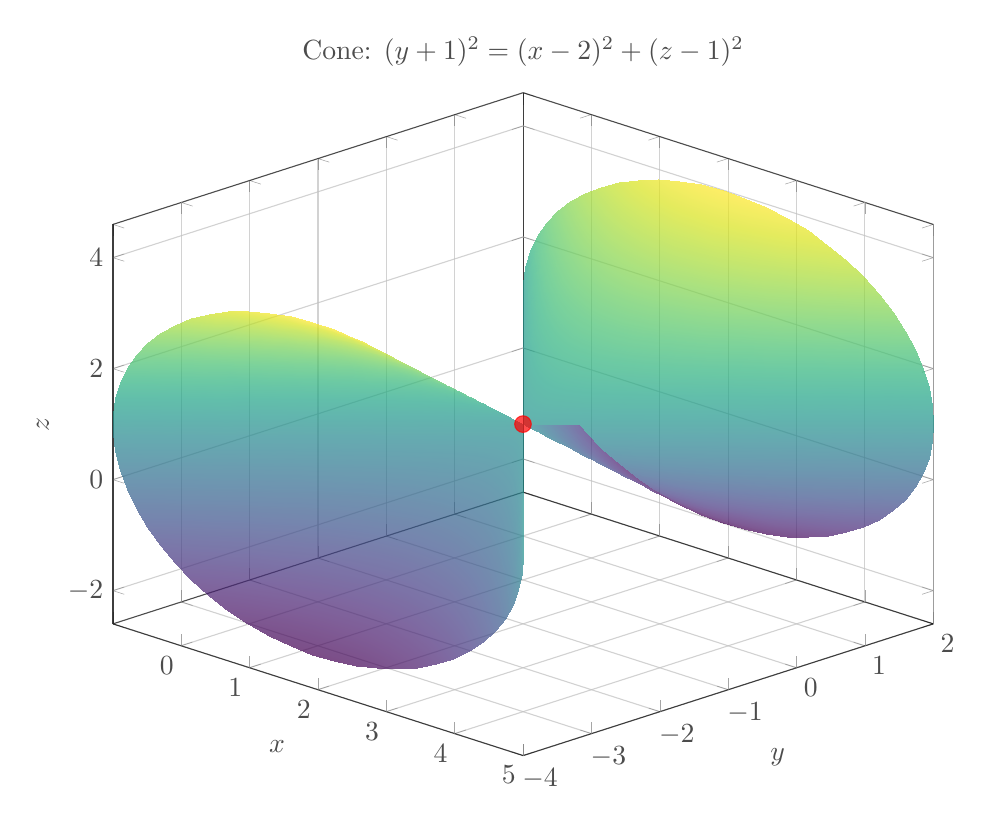
\begin{tikzpicture}
\begin{axis}[
    width=12cm,
    height=10cm,
    xlabel=$x$,
    ylabel=$y$,
    zlabel=$z$,
    title={Cone: $(y+1)^2 = (x-2)^2 + (z-1)^2$},
    view={45}{25},
    grid=major,
    colormap/viridis,
    shader=interp,
    opacity=0.7,
]
% Upper cone
\addplot3[
    surf,
    domain=0:3,
    y domain=0:360,
    samples=30,
    samples y=60,
] 
({2 + x*cos(y)}, {-1 + x}, {1 + x*sin(y)});

% Lower cone
\addplot3[
    surf,
    domain=0:3,
    y domain=0:360,
    samples=30,
    samples y=60,
] 
({2 + x*cos(y)}, {-1 - x}, {1 + x*sin(y)});

% Vertex point
\addplot3[
    only marks,
    mark=*,
    mark size=3pt,
    red,
] coordinates {(2, -1, 1)};

\end{axis}
\end{tikzpicture}
\end{document}